\documentclass[10pt]{article}

\usepackage[margin=19mm]{geometry}
\usepackage{amsmath}
\usepackage{booktabs}
\usepackage{float}
\usepackage{graphicx}
\usepackage{microtype}
\usepackage[T1]{fontenc}
\usepackage{lmodern}

\title{Channel, OFDM Configuration, and Receiver Choice: A One-Frame Illustration}
\author{}
\date{}

\begin{document}
\maketitle
\vspace{-2.5em}

Underwater acoustic channels vary with time and location, and receiver
performance depends on both the channel and the selected physical-layer
parameters. We consider one frame to illustrate why receiver results must be
read together with the channel and configuration. This experiment supports an
explanation of the four tested conditions; it does not support a general rule
for selecting a receiver.

\section{Experiment}

We used one frame from hydrophone~1 of the Red-1 and Blue-1 captures.
The Signal-to-Noise Ratio (SNR) was 20~dB, and we used seed~4 and snapshot~1.
Every condition used cyclic prefix length~64, code rate~$1/4$, outer pilot
spacing~6, and inner pilot spacing~8. We changed the Orthogonal Frequency
Division Multiplexing (OFDM) transform length $N$ between 512 and 1024.

Five receivers processed the same payload, encoded bits, transmitted waveform,
replay output, and noise realization within each condition. Hence differences
between receiver rows within one condition arise after this common input.
All five receivers use Low-Density Parity Check (LDPC) decoding. The five exact
receiver labels are OFDM+LDPC, Partial-FFT+LDPC, JUNA-Iterative, profiled
JUNA-$(C,z)$, and JUNA-Direct-$(C,z)$.
% Generated by build_jcm386_figures.py from demo_manifest.json.
All five receivers use the same clean JunaCore source tree at commit \texttt{827bbb217e71}. That tree retains the shared carrier-offset and duration acquisition from commit \texttt{261a4418327b} and adds the tested Direct $C,z$ receiver.


The Partial-FFT+LDPC receiver used six Partial-FFT bands for Red-1 and 16
Partial-FFT bands for Blue-1. Hence the channel and $N$ alone cannot explain
the change between Red-1 and Blue-1.

\section{Physical configuration}

We first compare the same numerical settings in physical time. The useful
symbol and cyclic prefix durations are
\[
  T_s=\frac{N}{B}, \qquad T_{\mathrm{cp}}=\frac{N_{\mathrm{cp}}}{B},
\]
where $T_s$ is the useful symbol duration, $T_{\mathrm{cp}}$ is the cyclic
prefix duration, $N$ is the transform length, $N_{\mathrm{cp}}$ is the cyclic
prefix length, and $B$ is the bandwidth. These durations increase when
the same number of samples occupies a smaller bandwidth.

Figure~\ref{fig:physical-configuration} shows that the same numerical $N$ and
cyclic prefix length do not give the same physical durations in Red-1 and
Blue-1. The Blue-1 useful symbol at $N=512$ is close in duration to the Red-1
useful symbol at $N=1024$.

\begin{figure}[H]
  \centering
  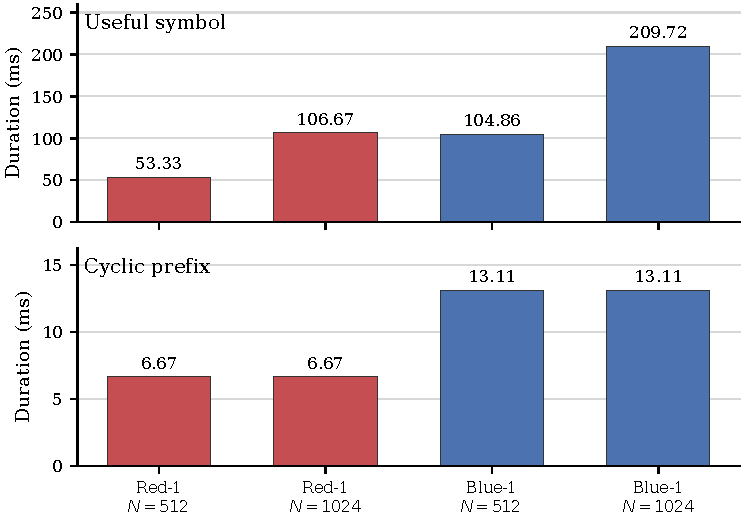
\includegraphics[width=\columnwidth]{figures/fig1_physical_configuration.pdf}
  \caption{Useful symbol and cyclic prefix durations for the four tested
  conditions. Red-1 used 9600~Hz bandwidth, while Blue-1 used 4882.8125~Hz.}
  \label{fig:physical-configuration}
\end{figure}

\section{Results}

We measure each receiver using its payload Bit Error Rate (BER),
$\mathrm{BER}=e/n$, where $e$ is the number of payload bit errors and $n$ is
the number of payload bits. A smaller BER means that fewer payload bits were
decoded incorrectly.

Figure~\ref{fig:ber} uses a common vertical scale in all four panels. The
number above each bar gives the exact payload bit error count, including zero.
Table~\ref{tab:one-frame-results} gives the same counts with the payload size
for each condition.

\begin{figure}[H]
  \centering
  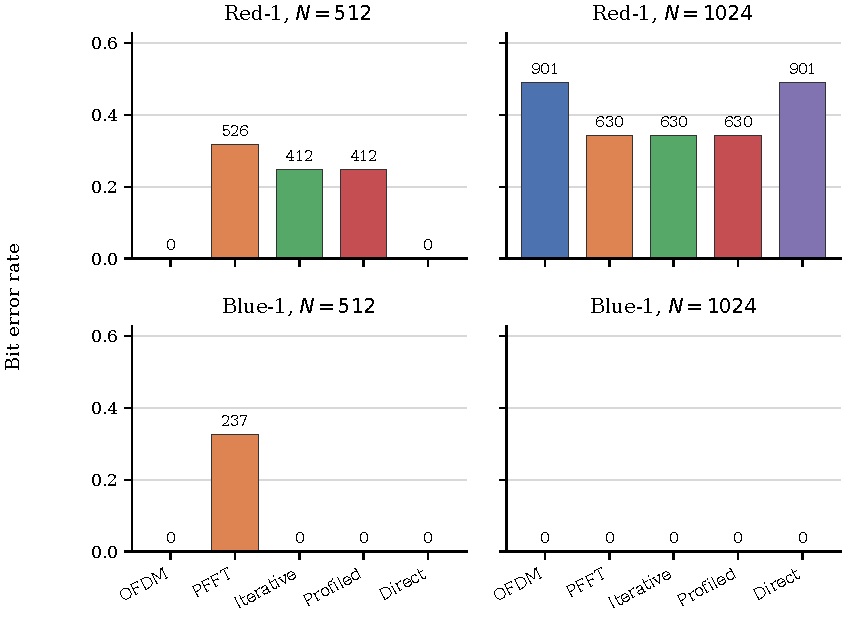
\includegraphics[width=0.88\columnwidth]{figures/fig2_bit_error_rate.pdf}
  \caption{Payload BER for the five receivers in each tested condition. The
  panels have identical vertical limits, and each label gives the corresponding
  number of payload bit errors.}
  \label{fig:ber}
\end{figure}

% Generated by build_jcm386_figures.py from frame_results.csv.
\begin{table}[H]
\centering
\caption{Payload bit errors in the one-frame experiment. Bold entries indicate an error-free frame.}
\label{tab:one-frame-results}
\setlength{\tabcolsep}{2.2pt}
\resizebox{\columnwidth}{!}{%
\begin{tabular}{lrrrrrrr}
\toprule
Capture & $N$ & Payload & OFDM & PFFT & Iterative & Profiled & Direct \\
\midrule
Red-1 & 512 & 1653 & \textbf{0} & 526 & 412 & 412 & \textbf{0} \\
Red-1 & 1024 & 1839 & 901 & 630 & 630 & 630 & 901 \\
Blue-1 & 512 & 726 & \textbf{0} & 237 & \textbf{0} & \textbf{0} & \textbf{0} \\
Blue-1 & 1024 & 726 & \textbf{0} & \textbf{0} & \textbf{0} & \textbf{0} & \textbf{0} \\
\bottomrule
\end{tabular}%
}
\end{table}


The results for the four conditions are as follows.
% Generated by build_jcm386_figures.py from frame_results.csv.
At Red-1 with $N=512$, OFDM+LDPC and JUNA-Direct-(C,z) decoded the 1653-bit payload without an error.
The error counts were 526, 412, and 412 for Partial-FFT+LDPC, JUNA-Iterative, and profiled JUNA-(C,z), respectively.
At Red-1 with $N=1024$, no receiver decoded the 1839-bit payload without an error.
The error counts were 901, 630, 630, 630, and 901 for OFDM+LDPC, Partial-FFT+LDPC, JUNA-Iterative, profiled JUNA-(C,z), and JUNA-Direct-(C,z), respectively.
At Blue-1 with $N=512$, OFDM+LDPC, JUNA-Iterative, profiled JUNA-(C,z), and JUNA-Direct-(C,z) decoded the 726-bit payload without an error.
The error count was 237 for Partial-FFT+LDPC.
At Blue-1 with $N=1024$, all five receivers decoded the 726-bit payload without an error.
JUNA-Direct-(C,z) matched OFDM+LDPC in all four conditions because it retained the OFDM+LDPC (Standard) result.
The Standard result passed the cyclic redundancy check (CRC) in Red-1 at $N=512$ and in both Blue-1 conditions.
In Red-1 at $N=1024$, eight Direct steps ran, but no CRC-valid candidate replaced Standard.
This run therefore contains no Direct rescue.


\pagebreak
Frame success requires zero payload bit errors and no decoding failure. For
this illustration, $r$ is a configured one-second payload budget, not
throughput calculated using the waveform duration. We calculate it as
\[
  r=\begin{cases}
  n/B, & \text{for a successful frame},\\
  0,   & \text{for a failed frame},
  \end{cases}
\]
where $r$ is the configured one-second effective payload rate, $n$ is the
payload size, and $B$ is the bandwidth. This definition makes the cost of a
single residual error visible, because a failed frame contributes no payload
rate. The actual waveform durations in all four conditions were less than one
second.

\begin{figure}[H]
  \centering
  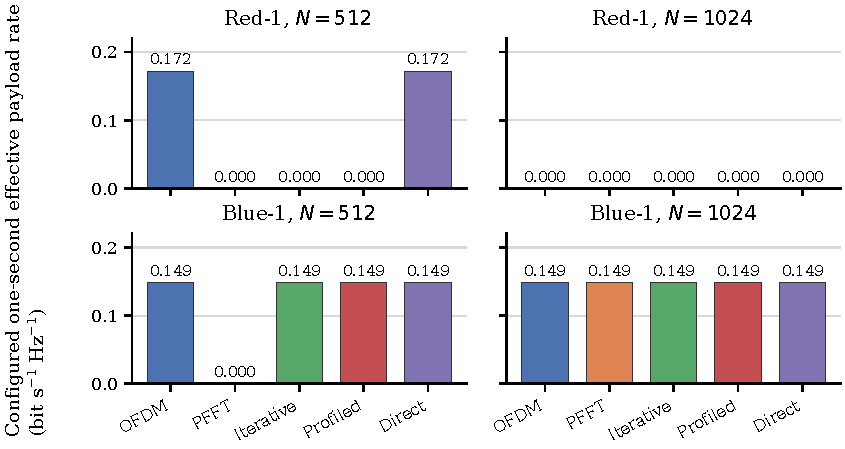
\includegraphics[width=0.90\columnwidth]{figures/fig3_effective_payload_rate.pdf}
  \caption{Configured one-second effective payload rate for the same four
  conditions. A receiver contributes payload rate only when it decodes the
  complete frame without an error.}
  \label{fig:effective-rate}
\end{figure}

Figures~\ref{fig:ber} and~\ref{fig:effective-rate} show that both the BER
ordering and the set of successful receivers change across the four
conditions. Thus the receiver with the smallest BER in one condition need not
have the smallest BER in another condition.

\section{Limits}

We used one frame per condition, one capture per channel, one hydrophone, one
SNR, and one seed. Hence these data cannot establish a rule for selecting a receiver,
an association, a cause, or an error floor. Estimating an error floor requires
multiple SNR values, while a BER distribution requires multiple frames.

The five rows within each condition share their payload, waveform, replay
output, and noise realization; they form paired receiver comparisons, not
independent channel observations. Relating receiver performance to channel
conditions requires matched captures, hydrophones, SNR values, seeds, and
frames.

\section{Conclusion}

We considered five receivers under two OFDM configurations on Red-1 and
Blue-1. The $N=512$ and $N=1024$ results differed between Red-1 and Blue-1.
The same numerical settings also produced different physical
durations because the bandwidths differed.

Although this one-frame result explains the tested comparison, it does not
show that one receiver is generally better. Receiver choice and modulation
scheme must therefore be evaluated together under matched channel conditions.

\end{document}
